\section{Implementation of the algorithm}
We start by presenting the broad implementation of the Metropolis algorithm, before showing how we adapt it to each specific model.
\subsection{The Metropolis algorithm}
In order to make the models evolve in time, which is necessary to observe their dynamics, we use the well-known metropolis algorithm \cite{Metropolis1953}. For models with a defined Hamiltonian, the Metropolis algorithm proceeds as follows:
\begin{enumerate}
    \item Start from an initial configuration $\{S_i\}$.
    \item Repeat $N$ times:
    \begin{enumerate}[label=\alph*.]
        \item Pick a random spin $S_k$ and compute the energy change $\Delta E_k$
              upon flipping it.
        \item If $\Delta E_k \leq 0$, accept the flip.
        \item Else, draw a random number $r \sim \mathcal{U}([0,1])$
              and accept the flip if $r \leq e^{-\beta \Delta E_k}$.
    \end{enumerate}
    \item Repeat Step 2 for $N_{\text{sweeps}}$ sweeps.
\end{enumerate}
Where $N$ is the number of spins, $\beta$ is the inverse temperature,
and $N_{\text{sweeps}}$ is the number of sweeps, where one sweep consists of
$N$ successive single-spin flip attempts.\\
This algorithm however becomes computationally demanding when one attempts to sample a large number of configurations. This situation occurs, for example, when looking for rare samples in the dynamics, or sampling many different initial conditions -- both of which we will try to explore during this internship. We thus need to find way of optimizing the implementation of the algorithm.

\subsection{First optimization: the bitwise arithmetic}
The first optimization in the implementation of the Metropolis algorithm is the use of bitwise arithmetic. The main idea is to leverage the boolean representation as stored in our computers. The typical object that we manipulate is called \texttt{Bits}: it is a collection of $n_\text{bits}=64$ boolean variables. In that way, we have the possibility to simulate $64$ evolutions of the same variable in parallel.
\begin{figure}[ht]
\centering
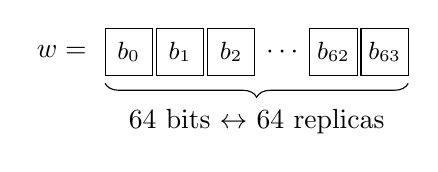
\begin{tikzpicture}
% Boîtes gauche : b_0 à b_2
\foreach \i/\label in {0/0, 1/1, 2/2} {
\draw (\i*0.65, 0) rectangle (\i*0.65+0.6, 0.6);
\node[font=\small] at (\i*0.65+0.3, 0.3) {$b_{\label}$};
}
% Points de suspension
\node at (3*0.65+0.3, 0.3) {$\cdots$};
% Boîtes droite : b_62, b_63
\foreach \i/\label in {0/62, 1/63} {
\draw (4*0.65 + \i*0.65, 0) rectangle (4*0.65 + \i*0.65+0.6, 0.6);
\node[font=\small] at (4*0.65 + \i*0.65+0.3, 0.3) {$b_{\label}$};
}
% Label gauche
\node at (-0.55, 0.3) {$w=$};
% Accolade en dessous
\draw[decorate, decoration={brace, amplitude=5pt, mirror}]
    (0, -0.1) -- (4*0.65+1*0.65+0.6, -0.1)
    node[midway, below=6pt] {64 bits $\leftrightarrow$ 64 replicas};
\end{tikzpicture}
\caption{A \texttt{Bits} $w$ encoding 64 parallel replicas. Each bit $b_i$ carries the state of replica $i$.}
\label{fig:bitword}
\end{figure}

This structure is very convenient to represent binary variable such as the spins of the system. The boolean representation $b_i \in \{0,1\}$ of a spin $s_i \in \{-1,+1\}$ is given by $b_i = (s_i+1)/2$. In that way, we are able to implement several replicas of the full spin system in a set of \texttt{Bits} $\{S_i\}$, each encoding the replicas of the associated spin, as shown in Figure~\ref{fig:spins_Bits}.

\begin{figure}[H]
\centering
\def\svgwidth{0.28\linewidth}
\input{pictures/spins_Bits.pdf_tex}
\caption{Bitwise implementation of a spin system. Each replica of the system is obtained by selecting the corresponding replica in each spin.}
\label{fig:spins_Bits}
\end{figure}



The limitation of $n_\text{bits}$ to $64$ is directly related to the architecture of modern CPUs \cite{} \noteBastien{I need some sources here}. This limit may in principle be extended up to $512$ bits
using SIMD instructions, but that requires the use of new object type in our code. This will be left for further discussion.\\



\begin{figure}[h]
\centering
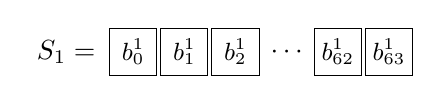
\begin{tikzpicture}
% Boîtes gauche : b_0 à b_2
\foreach \i/\label in {0/0, 1/1, 2/2} {
\draw (\i*0.65, 0) rectangle (\i*0.65+0.6, 0.6);
\node[font=\small] at (\i*0.65+0.3, 0.3) {$b_{\label}^1$};
}
% Points de suspension
\node at (3*0.65+0.3, 0.3) {$\cdots$};
% Boîtes droite : b_62, b_63
\foreach \i/\label in {0/62, 1/63} {
\draw (4*0.65 + \i*0.65, 0) rectangle (4*0.65 + \i*0.65+0.6, 0.6);
\node[font=\small] at (4*0.65 + \i*0.65+0.3, 0.3) {$b_{\label}^1$};
}
% Label gauche
\node at (-0.55, 0.3) {$S_1=$};
\label{fig:bitword}
\end{tikzpicture}
\end{figure}
\subsection{Second Optimization: Shared random numbers}
\subsection{Structure of the code}
